Die Serverzuständigkeiten lassen sich in folgende Aspekte zusammenfassen:
\begin{itemize}
\item Empfangen und Beantworten der Clientanfragen
\item Routing der Anfragen zu den entsprechenden Abhandlungsroutinen
\item Überprüfen der Identität des Clients
\item Kommunikation zur Datenbank für die persistente Speicherung der Zustände der Nutzer und ihrer Präferenzen, Swipes und Matches.
\item Matching-Algorithmus
\end{itemize} 

\noindent
In den folgenden Unterkapitel wird auf die Einrichtung des Node.js-Webservers und der MongoDB-Datenbank, auf die Erstellung der sicheren Kommunikationsschnittstelle und auf die Implementierung der serverzuständigen Funktionalitäten eingegangen.

\subsubsection{Bereitstellung des Webservers}
Zunächst wird das Node.js-Installationspaket aus der offiziellen Seite der Hersteller heruntergeladen und ausgeführt. Hierbei werden sowohl die Laufzeitumgebung für Node.JS, als auch der npm package manager installiert (Siehe nächste Abbildung). 
Zusätzlich wird bei der Installation ausgewählt, dass Node.js sowie npm und dessen Module zu den Umgebungsvariablen hinzugefügt werden. Dabei werden Variablen unter ihrem Applikationsnamen gespeichert und ihre entsprechende Datei-Pfade hinterlegt.
Über den Zugriff auf diese Umgebungsvariable ist ein schneller Zugriff über ein Terminal beziehungsweise einer anderen Applikation gewährleistet.


\begin{figure}[tbt]
\centering
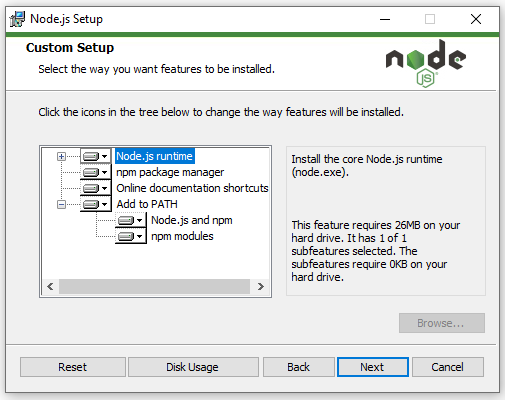
\includegraphics[width=8cm]{images/nodejs_install.png}
\caption{Node.JS Installation}
\label{fig:installation_nodejs}
\end{figure}

\noindent
Nach der Installation von Node.js (siehe Abbildung \ref{fig:installation_nodejs}) kann das Projekt mithilfe des Befehls „npm init“ im Terminal initializiert werden. 
Hier werden nacheinander Input für relevante Projektaspekte wie dem Projektnamen, der Initialversion, der Startprogrammdatei oder dem GIT-Repository abgefragt.  
Im Anschluss wird im aktuellen Verzeichnis eine Datei „package.json“ erstellt,  bei der es sich um eine Manifest-Datei im JSON- Format handelt, die unter anderem die benötigten Pakete sowie dessen Version, als auch projektspezifische Meta-Informationen wie den Projektnamen, der Projektversion, der Projektbeschreibung und dem Author enthält.
\newline
Im Anschluss an die Initialisierung werden die benötigten Pakete installiert. Dafür wird der Befehl „npm install“ in Kombination mit dem angeforderten Modul genutzt. 
Nach der ersten Installation eines Moduls wird im Hauptverzeichnis des Projekts automatisch ein Ordner „node\_modules“ erzeugt. Dieser enthält die Quelldaten der Node.js-Module. 
\newline
Da die Funktionalität, die nodemon bietet, nur in der Entwicklung benötigt wird, wird in der Datei „package.json“ ein Entwicklungsskript „devStart“ definiert. 
Skripte erlauben das automatische Starten von anderen Applikationen. Über „npm run“ in Kombination mit dem auszuführenden Skript wird die Hauptapplikation über die Datei, die im package.json unter „main“ hinterlegt ist, zusammen mit den Applikationen, die im package.json unter dem entsprechenden Skript aufgezählt sind, gestartet.
\newline
Als Applikationsstartpunkt wird die Datei „server.js“ erzeugt und im package.json unter main hinterlegt. 

\begin{lstlisting}[caption=Datei package.json, label=lst:packagejson]
{
  "name": "StreamSwipeServer",
  "version": "1.0.0",
  "description": "Our Backend-Server for the StreamSwipe Mobile Application",
  "main": "server.js",
  "scripts": {
    "start": "",
    "devStart": "nodemon"
  },
  "author": "Robin Meckler, Vincent Schreck, Leon Gieringer",
  "license": "-",
  "dependencies": {
    "express": "^4.17.1",
    "firebase-admin": "^9.5.0",
    "mongoose": "^5.11.17",
    "node-cron": "^2.0.3",
    "dotenv": "^8.2.0"
  },
  "devDependencies":{
    "nodemon": "^2.0.7"
  }
}
\end{lstlisting}

\subsubsection{Sichere Kommunikation}
\label{sec:SichereKommunikation}
Das http-Modul ermöglicht eine Kommunikation über das http-Protokoll.\\
 
\begin{lstlisting}[caption=Einfache Verbindung, label=lst:nodejs_easyconnection]
{
 const app = express();
 app.use(express.json()); 
 var httpServer = http.createServer(app);
 httpServer.listen(process.env.HTTP_PORT, () => 
 console.log("HTTP-Server started on " + process.env.HTTP_PORT));
}
\end{lstlisting}

\noindent
Dabei werden jedoch die Daten unverschlüsselt versendet. Um ausreichend Datenschutz zu gewährleisten, wird stattdessen das https-modul genutzt. \footnote{Siehe Dokumentation: \url{https://nodejs.org/api/https.html}, letzter Zugriff: 24. April 2021}
\newline
Benötigt für einen HTTPS-Server werden ein Sicherheitszertifikat und ein privater Schlüssel, die zunächst mithilfe des Tools OpenSSL erzeugt werden.  
Dabei ist zu beachten, dass während der Entwicklungsphase das Zertifikat nicht von einer zuständigen Zertfikatsstelle signiert wird und somit von anderen Gegenstellen nicht akzeptiert wird.
\newline
In der Anwendung wird zunächst ein Objekt 'httpsOptions' erzeugt, dass unter dem Attribut 'cert' das generierte Sicherheitszertifikat und unter dem Attribut 'key' den privaten Schlüssel enthält. Anschließend wird über die Funktion 'createServer' des https-Objekts der https-Server gestartet, woraufhin ein Objekt vom Typ https.Server zurückgegeben wird \footnote{Siehe Dokumentation:  \url{[https://nodejs.org/api/https.html\#https_class_https_server]}, letzter Zugriff: 24. April 2021}. 
Diesem Serverobjekt wird über seine Methode 'listen' aufgefordet, auf eingehende Nachrichten in dem als Parameter übergebenem Port einzugehen.\\

\begin{lstlisting}[caption=Gesicherte Verbindung, label=lst:nodejs_safeconnection]
{
 ...
 const https = require("https");
 const httpsOptions = {
  cert: fs.readFileSync('sslcert/server.crt', 'utf8'),
  key: fs.readFileSync('sslcert/server.key', 'utf8')
 }
 var httpsServer = https.createServer(httpsOptions, app);
 httpsServer.listen(process.env.HTTPS_PORT, () => {console.log("HTTPS - 	Server started on " + process.env.HTTPS_PORT)});
}
\end{lstlisting}


\subsubsection{Datenbankverbindung}
Wie bereits erwähnt, wird das Modul „mongoose“ für die Verbindung mit der MongoDB-Datenbank verwendet. 
Da der Quellcode in anderen Dateien hinterlegt ist, muss für den Zugriff auf dessen Funktionalitäten das entsprechende Modul zunächst inkludiert werden. Dazu wird die require-Methode aufgerufen, die ein Objekt zurückgibt, dass die aus dem Modul exportierten Methoden enthält und im Folgenden als Variabel mit dem Namen „mongoose“ gespeichert wird. 
\newline
Über die connect-Methode des zurückgelieferten Objekts wird nun bei Parameterübergabe der URL der Datenbank versucht, eine Verbindung aufzubauen.  
Dabei wird unter der Objekt-Membervariabel  „connection“ ein Objekt vom Typ „Connection“ hinterlegt, über das bei erfolgreicher Verbindung mit der Datenbank kommuniziert werden kann und das nachfolgend unter der Variabel „database“ abgespeichert ist.\\

\begin{lstlisting}[caption=Verbindung zur MongoDB-Datenbank, label=lst:mongodbconnection]
{
 const mongoose = require('mongoose');
 let database = null;

 async function startDatabase() {
  await mongoose.connect(process.env.DATABASE_URL, 
   {useNewUrlParser: true,
   useUnifiedTopology: true}); 
  database = mongoose.connection;
  database.on('error',(error) => console.log(error));
  	database.on('open',(error) => console.log('Connected to DB'))}

 async function getDatabase() {
 if (!mongoose.connection) await startDatabase();
  return database; }

 module.exports = {
  getDatabase,
  startDatabase }
}
\end{lstlisting}

\subsection{Datenbank}
\subsubsection{Datenbankmodelle und Schemata}

Ein Model in Mongoose ist ein aus einer Schemadefinition erstellter Konstruktor, aus denen Objekte instanziiert werden können. Diese Instanzen stehen in direkter Verbindung zu den jeweiligen Collections der verbundenen Datenbank und enthalten Methoden für die persistente Speicherung, Bearbeitung oder Löschung.
\newline
Folgender Code zeigt den Aufbau des Schemas für die Swipe-Collection. 

\begin{lstlisting}[caption=Swipe Schema und Model, label=lst:modelswipe]
	const mongoose = require('mongoose')

	const swipeSchema = new mongoose.Schema({
    uid: {
        type: String,
        required: true
    },
    swipes :
     [{ movieid: { type: String },
        swipeaction: {type: Number}}]
	})

	module.exports = mongoose.model('Swipe',swipeSchema)
\end{lstlisting}

Die einzelnen Schemata wurden nach dem im Konzept beschriebenen Aufbau [TODO] für jede Collection in separaten Dateien unter dem Verzeichnis '/database/models' erstellt. Jede Datei exportiert dabei das aus dem zugehörigen Schema erzeugten Model.

\begin{figure}[h]
\centering
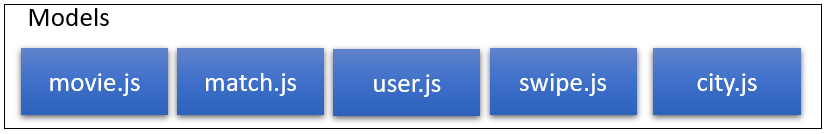
\includegraphics[width=8cm]{images/modelsstruktur.PNG}
\caption{Node.js Server - Models Struktur}
\end{figure}


\subsubsection{Datenbankzugriff}                   
Für den Datenzugriff auf die Datenbank wurden zu jeder Collection Service-Module unter dem Verzeichnis '/services' erstellt, die entsprechenden Zugriff gewähren. Dafür wurden innerhalb der Service-Modulen  die benötigten Zugriffsfunktionen implementiert (siehe Abbildung \ref{fig:node_service_structure}).

\begin{figure}[tbt]
\centering
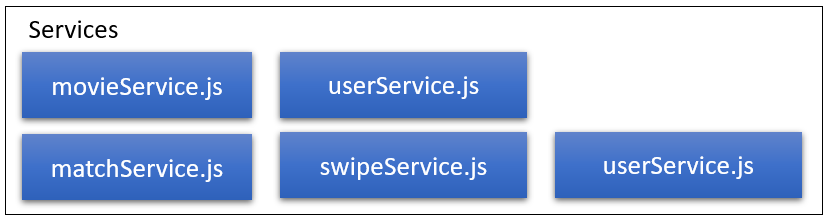
\includegraphics[width=12cm]{images/serviceStruktur.PNG}
\caption{Node.js Server - Services Struktur}
\label{fig:node_service_structure}
\end{figure}


%
%              Movie
%                   Service
%

\paragraph{Movie Service}
Die Funktionen des Moduls movieService.js bieten innerhalb der Projektumgebung den Zugriff auf bestimmte Operationen, die  auf die Collection movies angewandt werden. Der Funktionsspektrum begrenzt sich für diesen Service auf die Funktion 'FindMovieExcept'.

\noindent
\textbf{FindMoviesExcept:}
Diese Funktion erhält als Parameter 'excludedMovies' eine Liste von MovieID's und als Parameter 'amount' einen Integerwert.
Über die Find-Funktion des importierten Movie-Models wird eine über den Wert von 'amount' begrenzte Anzahl an Movie-Dokumenten ausgelesen, deren ID nicht in der übergebenen 'excludedMovies'-Liste vorhanden sind. Für das Filtern wird die 'nin'-Operation verwendet.\footnote{Siehe Dokumentation: \url{https://docs.mongodb.com/manual/reference/operator/query/nin/}, letzter Zugriff: 26. April 2021}

Sollte die Datenbank bei der Datenauslese ein Fehler zurückgeben, wird dieser über den try-catch-Block gefangen und an im Aufrufstack überliegende Funktion über das Schlüsselwort throw weitergeleitet.\\

\begin{lstlisting}[caption=movieService.js - FindMoviesExcept, label=lst:findmoviesexcept]
const Movie = require('../database/models/movie')

async function FindMoviesExcept(excludedMovies, amount) {
    var movies;

    try{ 
    movies = await Movie.find({ id: { $nin: excludedMovies }}).limit(amount); }
    }
    catch(err){throw err;}

    return movies;
}

module.exports.FindMoviesExcept = FindMoviesExcept;
\end{lstlisting}


%
%              User
%                   Service
%

\paragraph{User Service}
Die Funktionen des Moduls userService.js bieten innerhalb der Projektumgebung den Zugriff auf bestimmte Operationen, die auf die Collection User angewandt werden. Dieser Service import das User-Model.\\

\noindent
\textbf{CreateUser:}
Die Funktion erhält sämtliche Eigenschaften, die im User-Schema beschrieben sind, als Parameter. Diese Funktion wird in der Projektumgebung in Zusammenhang mit mindestens einer weiteren datenbankzugreifenden Funktion aufgerufen. Im Sinne einer Transaktion müssen sie als atomare Operation ausgeführt werden, um den Datenbestand konsistent zu halten. Daher wird ein Session-Objekt als Parameter mitgeliefert. Innerhalb der Funktion wird über die Create-Funktion des importierten User-Models ein neuer Eintrag in der User-Collection der Datenbank erstellt.

\begin{lstlisting}[caption=User Service - CreateUser, label=lst:userservicecreateuser]
async function CreateUser(uid, swipeid, matchid, city, malewanted, femalewanted, diversewanted, mygender, session) {
    try {
        return (await User.create([{
            _id: mongoose.Types.ObjectId(),
            uid: uid,
            _swipeid: swipeid,
            _matchid: matchid,

            city: city,
            malewanted: malewanted,
            femalewanted: femalewanted,
            diversewanted: diversewanted,
            mygender: mygender
        }
        ], { session: session }))[0];
    }
    catch (Exception) {
        throw Exception;
    }
}
\end{lstlisting}

\noindent
\textbf{CheckExistence:}
Die Funktion prüft darauf, ob innerhalb der User-Collection ein User mit entsprechendem Wert für die Eigenschaft 'uid', die als Parameter übergeben wird und gibt entsprechend den boolschen Wert 'true' bei Vorhandensein beziehungsweise 'false' bei Nicht-Vorhandensein zurück.\\

\begin{lstlisting}[caption=User Service - CheckExistence, label=lst:userservicecheckexistence]
async function CheckExistence(uid) {
    return await User.exists({ uid: uid });
}
\end{lstlisting}

\noindent
\textbf{GetCityFromUser:}
Die Funktion gibt den Eintrag der Eigenschaft 'city' eines Dokuments zurück, dessen 'uid'-Attribut mit dem übergebenen 'uid'-Parameter übereinstimmt.\\

\begin{lstlisting}[caption=User Service - CheckExistence, label=lst:userservicecheckexistence]
async function GetCityFromUser(uid) {
    try {
        var user = await User.findOne({ 'uid': uid });
        if (user) {
            return user.city;
        }
        else throw { message: "No user Found" + uid };
    }
    catch (err) { console.log(err); throw err; }
\end{lstlisting}

\noindent
\textbf{ChangeCityFromUser:}
Die Funktion führt ein Update auf einem User-Dokument aus, dessen 'uid'-Eigenschaft mit dem gleichnamigen übergebenemen Parameter übereinstimmt. Dabei wird die 'city'-Eigenschaft innerhalb des User-Dokuments auf den Wert des gleichnamigen Parameters aktualisiert.\\

\begin{lstlisting}[caption=User Service - ChangeCityFromUser, label=lst:userservicechangecityfromuser]
async function ChangeCityFromUser(uid, city, session) {  
   try {
        if (CheckExistence(uid)) {
            await user.UpdateOne(
                { 'uid': uid },
                { city: city },
                { session: session });
        }
        else throw { message: "No User Found" + uid }
    }
    catch (err) { console.log(err); throw err; }
\end{lstlisting}

\noindent
\textbf{ChangeGenderWantedFromUser:}
Die Funktion erfüllt die gleiche Funktionalität wie die ChangeCityFromUser-Funktionalität mit dem Unterschied, dass statt der 'city'-Eigenschaft die Eigenschaft 'malewanted','femalewanted' und 'diverswanted' aktualisiert werden.\\

\noindent
\textbf{ChangeGenderFromUser:}
Die Funktion erfüllt die gleiche Funktionalität wie die ChangeCityFromUser-Funktionalität mit dem Unterschied, dass statt der 'city'-Eigenschaft die 'mygender'-Eigenschaft aktualisiert wird.\\


%
%              Match
%                   Service
%


\paragraph{Match Service}
Die Funktionen des Moduls matchService.js bieten innerhalb der Projektumgebung den Zugriff auf bestimmte Operationen, die auf die Collection matches angewandt werden. Dieser Service import das Match-Model.

\noindent
\textbf{CreateUserMatchDocument:}
Die Funktion überprüft zunächst, ob ein Match-Dokument mit übergebener 'uid'-Eigenschaft bereits existiert. Ist dies nicht der Fall, wird ein neues Match-Dokument in der matches-Collection erzeugt.\\

\begin{lstlisting}[caption=Match Service - CreateUserMatchDocument, label=lst:matchserviceCreateUserMatchDocument]
async function CreateUserMatchDocument(uid, session) {
    if (!(await Match.exists({ uid: uid }))) {
        try {
            return (await Match.create([{
                _id: mongoose.Types.ObjectId(),
                uid: uid,
                swipes: []}
            ], { session: session }))[0];
        }
        catch (Exception) {
            throw Exception;
        }
    }
    else 
      throw { message: "Match already exists for " + uid 		};
    
}
\end{lstlisting}

\noindent
\textbf{CheckMatchExists:}
Die Funktion überprüft, ob ein Match-Dokument existiert, welches den übergebenen 'uid'-Eigenschaftswert hat sowie innerhalb seiner 'supermatches'- oder 'normalmatches'-Liste die übergebene 'matchedUid' enthält. Zurück wird ein entsprechender boolescher Wert geschickt. 

\begin{lstlisting}[caption=Match Service - CreateUserMatchDocument, label=lst:matchserviceCreateUserMatchDocument]
async function CheckMatchExists(uid, matchedUid, session) {
    try {
        var match = await Match.findOne({ uid: uid, 'supermatches.uid': matchedUid }).session(session)

        if (match) { return true; }
        else {
            var match = await Match.findOne({ uid: uid, 'normalmatches.uid': matchedUid }).session(session)

            if (match) return true;
            else return false;
        }
    }
    catch (err) { console.log(err); throw err; }
}
\end{lstlisting}

\noindent
\textbf{AddNormalMatchToUser:}
Die Funktion fügt der 'normalmatches'-Liste eines Match-Dokuments ein neues Objekt mit den Eigenschaften 'uid','matchUid' und 'movieid', die ihren Wert über die übergebenen Funktionsparameter erhalten. Des Weiteren wird das Attribut 'startedChat' und 'removed' jeweils mit dem booleschen Standardwert 'false' hinzugefügt. Außerdem wird die Eigenschaft 'newChanges' des Match-Dokuments auf true gesetzt.

\begin{lstlisting}[caption=Match Service - AddNormalMatchToUser, label=lst:matchserviceAddNormalMatchToUser]
async function AddNormalMatchToUser(uid, matchedUid, movieid, session) {
 try {
  if (Match.exists{ 'uid': uid }) {
   await Match.findOneAndUpdate(
    { 'uid': uid },
    { newChanges: true,
    $push: { normalmatches: { uid: matchedUid, 
                              movieid: movieid, 
                              startedChat: false, 
                              removed: false } }},
    { session: session });
    } else throw { message: "No Match Found" }; }
    catch (err) { console.log(err); throw err; }
}
\end{lstlisting}

\noindent
\textbf{AddSuperMatchToUser:}
Die Funktion unterscheidet sich von 'AddNormalMatchToUser' nur in dem Aspekt, dass ein neuer Eintrag in die 'supermatches'- statt der 'normalmatches'-Liste hinzugefügt wird.\\

\noindent
\textbf{GetMatches:}
Die Funktion empfängt eine 'uid' als Parameter und gibt ein entsprechendes Match-Dokument zurück, sofern es existiert.\\

\noindent
\textbf{SuperMatchMarkAsRemoved:}
Innerhalb der Funktion wird anhand des übergebenen 'uid' und 'matchesUid' der Eintrag in der 'supermatches'-Liste angepasst. Dabei wird der Wert für 'removed' auf true gesetzt. Ausserdem wird 'newChanges' des betroffenen Match-Dokuments auf true gesetzt.

\begin{lstlisting}[caption=Match Service - SuperMatchMarkAsRemoved, label=lst:matchserviceSuperMatchMarkAsRemoved]
async function SuperMatchMarkAsRemoved(uid, matchUid, session) {
 try {
  var match = await Match.findOneAndUpdate({ uid: uid, "supermatches.uid": matchUid },
  { "$set": { newChanges: true,
             "supermatches.$.removed": true }},
            { session: session });
  if (!match) {
   throw { message: "No Match Found:" + 
           uid + "matching: " + matchUid };}
 } catch (err) { console.log(err); throw err; }
}
\end{lstlisting}

\noindent
\textbf{NormalMatchMarkAsRemoved:}
Die Funktion unterscheidet sich von 'SuperMatchMarkAsRemoved' nur in dem Aspekt, dass der  Eintrag in der 'supermatches'- statt der 'normalmatches'-Liste angepasst wird.\\

\noindent
\textbf{MatchesReceived:}
Anhand einer übergebenen 'uid' und 'matchUid' wird die Eigenschaft 'newChanges' eines entsprechenden Match-Dokuments in der Match-Collection auf den booleschen Wert false gesetzt. 



%
%              Swipe
%                   Service
%

\paragraph{Swipe Service}
Die Funktionen des Moduls swipeService.js bieten innerhalb der Projektumgebung den Zugriff auf bestimmte Operationen, die auf die Collection swipes angewandt werden. Dieser Service import das Swipe-Model.\\

\noindent
\textbf{CreateUserSwipeDocument:}
Die Funktion erfüllt die gleiche Funktionalität wie die 'Create\-UserMatchDocument'-Funktionalität des Match-Services mit dem Unterschied, dass anstelle eines Match-Dokuments ein Swipe-Dokument in der swipes-Collection erstellt wird.\\

\noindent
\textbf{AddSwipe:}
Die Funktion erstellt zunächst ein swipe-Objekt mit den Eigenschaften 'movieid' und 'swipeaction' und entnimmt die Werte dafür aus den gleichnamigen übergebenen Parametern. 
Wenn ein Swipe-Dokument mit übergebener 'uid' existiert, wird überprüft, ob das Dokument in der 'swipes'-Liste bereits ein Eintrag mit entsprechender movieid enthält. Ist dies der Fall, wird die 'swipeaction'-Eigenschaft auf den Wert des übergebenene gleichnamigen Parameters aktualisiert. Ansonsten wird der Liste das zu Beginn erstellte 'swipe'-Objekt hinzugefügt. Letzlich wird das Swipe-Dokument über die Save-Funktion des Save-Models gespeichert.

\begin{lstlisting}[caption=Swipe Service - AddSwipe, label=lst:swipeserviceaddswipe]
async function AddSwipe(uid, movieid, swipeaction) {
 var swipe = { movieid: movieid, swipeaction: swipeaction };
 var dbSwipe;
 if (Swipe.exists({ 'uid': uid })) {
  try {
   dbSwipe = await Swipe.findOne({ 'uid': uid });

   //Ueberpruefe Vorhandensein des Swipes
   var index = dbSwipe.swipes.findIndex(x => x.movieid === movieid);

   if (index >= 0) {
    if (dbSwipe.swipes[index].swipeaction != swipeaction)
      dbSwipe.swipes[index].swipeaction = swipeaction; }
    else { dbSwipe.swipes.push(swipe); }
    dbSwipe.save(); 
    } catch (err) { throw err; }
  } else { throw "No Swipe available for this uid " + uid;}
  dbSwipe.save();
  return swipe;
}
\end{lstlisting}

\noindent
\textbf{RequestSwipes:}
Die Funktion empfängt eine 'uid' als Parameter und gibt ein entsprechendes Match-Dokument zurück, sofern es existiert.\\

\noindent
\textbf{RequestSuperlikeSwipes:}
Innerhalb dieser Funktion kommt es zum Einsatz einer Aggregation. 
Dabei kommt es zum Einsatz mehrerer Pipeline-Operatoren. []
% %TODO Link auf Tabelle 5 Aggregation Framework
Über den 'unwind'-Operator wird gesetzt, dass für jeden Listeneintrag innerhalb der 'swipes'-Liste neue Dokumente erzeugt werden, die in die nachfolgende Pipeline-Stufen weitergeleitet werden. Anhand des 'match'-Operators werden dann die neuen Dokumente gefiltert. Letzlich wird eine Liste von Swipes zurückgeschicht, die eine 'swipeaction' von 2 (entsprechend Superlike) aufweisen.

\begin{lstlisting}[caption=Swipe Service - RequestSuperlikeSwipes, label=lst:swipeserviceRequestSuperlikeSwipes]
async function RequestSuperlikeSwipes(uid) {
 var dbSwipe;
 if (Swipe.exists({ 'uid': uid })) {
  try {
   dbSwipe = await (await Swipe.aggregate([
    { $unwind: '$swipes' },
    { $match: { uid: uid,
                'swipes.swipeaction': 2 }},
    { $group: { _id: '$_id',
                swipes: { $push: { movieid: "$swipes.movieid",
                                  swipeaction: "$swipes.swipeaction" 
     }}}}]));
   if (dbSwipe.length > 0 && dbSwipe[0]) {
    return dbSwipe[0].swipes; }
   } catch (err) { throw err; } }
  else {throw { message: "Swipe uid not existing " + uid }; }
}
\end{lstlisting}

\noindent
\textbf{FindAllSwipedMoviesByUserID:}
Innerhalb dieser Funktion werden für eine übergebene 'uid' sämtlich movieid's zurückgeben, die in der 'swipes'-Liste des entsprechenden Swipe-Dokuments vorhanden sind.

\begin{lstlisting}[caption=Swipe Service - FindAllSwipedMoviesByUserID, label=lst:swipeserviceFindAllSwipedMoviesByUserID]
var swipedMovieIDs = [];
    
if (Swipe.exists({"uid": uid)) {
 try { var dbSwipe = await FindOne(uid);
  await dbSwipe.swipes.forEach(x => swipedMovieIDs.push(x.movieid));
 } catch (err) { throw err; }}
return swipedMovieIDs;
\end{lstlisting}


%
%              City
%                   Service
%
\paragraph{City Service}
Die Funktionen des Moduls cityService.js bieten innerhalb der Projektumgebung den Zugriff auf bestimmte Operationen, die auf die Collection cities angewandt werden. Dieser Service import das Swipe-Model.\\

\noindent
\textbf{GetAllInhabitedCities:}
Diese Funktion wird im Matching-Algorithmus aufgerufen. Er liefert sämtliche Städte, die mindestens zwei Nutzer aufzuweisen haben. 

\begin{lstlisting}[caption=City Service - GetAllInhabitedCities, label=lst:cityServiceGetAllInhabitedCities]
async function GetAllInhabitedCities() {
    var cities;
    try{ cities = await City.find({ user : {$exists:true},$where:'this.user.length>1'}) }
    catch (err) { throw err; }
    return cities;
}
\end{lstlisting}

\noindent
\textbf{AddUserToCity:}
Diese Funktion fügt einem 'City'-Dokument eine 'uid' hinzu.\\

\noindent
\textbf{RemoveUserFromCity:}
Diese Funktion entfernt eine 'uid' aus einem 'City'-Dokument.


\subsubsection{Controller} 
Controller sind für xy

\begin{figure}[h]
\centering
\includegraphics[width=8cm]{images/controllerStruktur.PNG}
\caption{Node.js Server - Controller Struktur}
\end{figure}

\paragraph{Movie Controller}

\begin{lstlisting}[caption=TODO, label=lst:TODO]
const SwipeService = require('../services/swipeService')
const MovieService = require('../services/movieService')
const FirebaseAdmin = require('../services/firebaseService')

exports.RequestMovies = async function(req, res){
   ...
}

\end{lstlisting}

\subparagraph{Request Movies}
\begin{lstlisting}[caption=TODO, label=lst:TODO]
    var uid; 
    const uidToken = req.body.uidtoken;
    
    //GET UID BY UIDTOKEN
    try
    {
        uid = await FirebaseAdmin.GetUID(uidToken);
    }
    catch(Exception)
    {
        res.status(401).json({title: "TOKEN ERROR", message: Exception});
        return;
    }

    var amount = req.body.amount;
    var includeSwiped = req.body.includeSwiped;
    var alreadyRequestedMovieIDs = req.body.alreadyRequestedMovieIDs;

    amount = RestrictAmount(amount); //Begrenzung auf max. 10 Filme

    //function variables
    var excludedMovieIDs = [];

    //Get already Swiped Movies
    var newMovies;
    if(includeSwiped === true)
    {
        var swipedMovieIDs;
        try{ swipedMovieIDs = await SwipeService.FindAllSwipesByUserID(uid) }
        catch(err){ res.status(400).json({message: err.message}) }

        excludedMovieIDs.push(...swipedMovieIDs);
    }

    //Get already Requested Movies
    if(alreadyRequestedMovieIDs !== undefined && alreadyRequestedMovieIDs != null)
    {
        await alreadyRequestedMovieIDs.forEach(element => excludedMovieIDs.push(element));
    }

    //Request Movies
    if(excludedMovieIDs.length > 0)
    {
        try{ newMovies = await MovieService.FindMoviesExcept(excludedMovieIDs,amount) } 
        catch(err){ res.status(400).json({message: err.message}) }
    }
    else
    {
        try{ newMovies = await MovieService.FindExactAmount(amount); } 
        catch(err){ res.status(400).json({message: err.message}) }
    }

    res.status(200).json(newMovies);
\end{lstlisting}


\paragraph{User Controller}
Im Folgenden werden..
\begin{itemize}
	\item CreateUser
	\item ChangeUser
	\item InfoUser
\end{itemize} 


\paragraph{Match Controller}
Im Folgenden werden..
\begin{itemize}
	\item RequestMatches
	\item DeleteSupermatch
	\item DeleteNormalmatch
	\item Received
	\item Trigger
\end{itemize} 



\paragraph{Swipe Controller}
Im Folgenden werden..
\begin{itemize}
	\item CreateSwipe
\end{itemize} 


\subsubsection{Routing} 
%\begin{figure}[h]
%\centering
%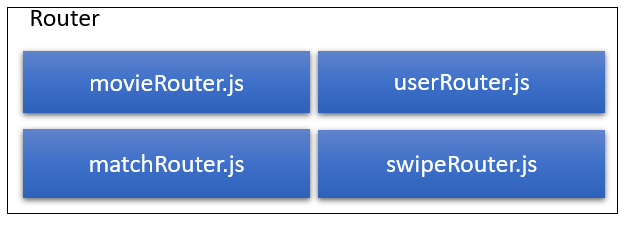
\includegraphics[width=8cm]{images/routestruktur.PNG}
%\caption{Node.js Server - Controller Struktur}
%\end{figure}
In der Server.js werden dem Express-Objekt 'app' die einzelnen Routen für die Weiterleitung der HTTPS-Anfragen an die entsprechenden Controller hinzugefügt. Dabei werden die zu den Anfragen gehörenden Request- und Response-Objekte als Parameter an die Controller übergeben.

\begin{lstlisting}[caption=Routing in server.js, label=lst:routingserver]
//Movies
const moviesRouter = require('./routes/movies')
app.use('/movies', moviesRouter)

//Users
const usersRouter = require('./routes/users')
app.use('/users', usersRouter)

//Matches
const matchesRouter = require('./routes/matches')
app.use('/matches', matchesRouter)

//Swipes
const swipesRouter = require('./routes/swipes')
app.use('/swipes', swipesRouter)

\end{lstlisting}

\paragraph{Movie Router}
Innerhalb des Movie Routers wird die '/movies/request' an die Funktion RequestMovie des Movie-Controller weitergeleitet.
\begin{lstlisting}[caption=Routing in movieRouter.js, label=lst:routingmovie]
// Require controller modules.
const MovieController = require('../controllers/movieController')

// Send Requests to MovieController
router.post('/request', MovieController.RequestMovies)
\end{lstlisting}

\paragraph{User Router}
Der User Router leitet '/users/create', '/users/change' und '/users/info' an die entsprechenden Funktionen des User-Controllers weiter.
\begin{lstlisting}[caption=Routing in userRouter.js, label=lst:routinguser]
// Require controller modules.
const UserController = require('../controllers/userController')

// Send Request to UserController
router.post('/create', UserController.CreateUser)
router.post('/change', UserController.ChangeUser)
router.post('/info', UserController.InfoUser)
\end{lstlisting}

\paragraph{Match Router}
Innerhalb des Match Routers werden die unten dargestellten URL's an die Funktion des Match-Controller weitergeleitet.

\begin{lstlisting}[caption=Routing in matchRouter.js, label=lst:routingmatch]
// Require controller modules.
const MatchController = require('../controllers/matchController')

// Send Request to MatchController
router.post('/request', MatchController.RequestMatches)
router.post('/deleteSupermatch',MatchController.DeleteSupermatch)
router.post('/deleteNormalmatch',MatchController.DeleteNormalmatch)
router.post('/received', MatchController.Received)
router.post('/trigger', MatchController.Trigger)
\end{lstlisting}


\paragraph{Swipe Router}
Der Swipe Router leitet '/swipes/create' an die entsprechende Funktionen des Swipe-Controllers weiter.

\begin{lstlisting}[caption=Routing in swipeRouter.js, label=lst:routingswipe]
// Require controller modules.
const SwipeController = require('../controllers/swipeController')

// Send Request to SwipeController
router.post('/create',  SwipeController.CreateSwipe )
\end{lstlisting}










\subsubsection{Weitere Backendfunktionalit"aten} 
Nachfolgend werden weitere Systemfunktionalitäten des Backends dargestellt.

\paragraph{Firebase-Service}
Um unberechtigte Zugriffe zu vermeiden, findet für die nutzerbezogenenen Anfragen eine Authentifizierung statt. Die erste Authentifizierung des Nutzers findet über den Login des Frontends in Firebase statt. Nachträglich muss bei Anfragen an den Webserver sichergestellt werden, dass der Nutzer weiterhin authentifiziert ist. Ohne diesen Vorgang könnte man sich über das Schicken einer willkürlich übermittelten Nutzer-Uid fälschlicherweise als anderer Nutzer ausgeben. Für den Zugriff auf die Firebase-Authentifizierungsfunktionen wird in die firebaseService.js-Datei das Modul 'firebase-Admin' importiert. \footnote{Siehe Dokumentation: \url{https://firebase.google.com/docs/admin/setup}, letzter Zugriff: 3. April 2021}

\noindent
\hangindent1cm
\textbf{Register:}
Um die Anwendung bei Firebase zu registrieren, wird die Funktion 'initializeApp' des Firebase-Moduls ausgeführt. 
Ein aus Firebase generierter Authentifizierungsschlüssel wird dabei für den Zugriff auf die StreamSwipe-Umgebung mitübergeben.
Die Register-Methode wird anschließend nach außen exportiert und zu Beginn des Serverstarts in der Server.js-Datei ausgeführt. 
\footnote{Siehe Dokumentation: \url{https://firebase.google.com/docs/admin/setup\#initialize-without-parameters}, letzter Zugriff: 3. April 2021}
   
\begin{lstlisting}[caption=Firebase-Service Register, label=lst:firebaseService Register]
var serviceAccount = require("../sslcert/streamswipe-firebase-adminsdk-uiyci-80bc08a5b2.json");
firebaseAdmin.initializeApp({
      credential: admin.credential.cert(serviceAccount),
        databaseURL: "https://streamswipe.firebaseio.com"
    });
\end{lstlisting}

\noindent
\hangindent1cm
\textbf{UID/TokenID-Dictionary:}
Um Zugriffszeiten auf die Firebase-Schnittstelle, werden in einem lokalen Dictionary aus Schlüsselwertpaaren der Zusammenhang zwischen TokenID und den UID samt ihrem Ablaufsdatum zwischen\-gespeichert.

\noindent
\hangindent1cm
\textbf{GetUID:}
Die Funktion erwartet einen Firebase Token als Parameter 'uidtoken', welcher an die Funktion 'verifyIdToken' des FirebaseAdmin-Objeekts weitergeleitet wird. Zurück wird ein Objekt gegeben, dass unter anderem die 'uid' des zum Token zugehörigen Nutzers und die Ablaufzeit schickt. Nach erfolgreichem Überprüfen, ob die 'uid' tatsächlich ein Wert übermittelt bekommen hat, wird das Paar aus UidToken und Uid samt Ablaufzeit in der UID/TokenID-Dictionary gespeichert.

\begin{lstlisting}[caption=Firebase-Service Register, label=lst:firebaseServiceRegister]
verifiedUid = await firebaseAdmin.auth().verifyIdToken(uidToken);
uid = verifiedUid.uid;
expireTime = verifiedUid.exp;
if(uid === undefined || uid == null) { throw {message: "No uid returned!"}; }
TokenIDDict[uidToken] = {uid,new Date(expireTime*1000)};
return uid;
... //Ende Try-Catch-Block
\end{lstlisting}
   
\noindent
\hangindent1cm
\textbf{RefreshList:}
Diese Funktion wird aufgerufen, um abgelaufene Token in der UID/TokenID-Dictionary zu löschen. Sie wird über das Modul TimedEvents periodisch aufgerufen. Dabei wird zu jedem Paar die aktuelle Uhrzeit und die Ablaufszeit verglichen. Stellt die Ablaufszeit ein größeren Wert dar, wird das Schlüsselwertpaar aus der Dictionary entfernt.

\paragraph{Timed Events}
Über das 'node-cron'-Modul \footnote{Siehe Dokumentation: \url{//https://www.npmjs.com/package/node-cron}, letzter Zugriff: 26. April 2021}
können zeitlich definierte und periodische Funktionen ausgeführt werden. Dafür wird das 'node-cron'-Modul in die TimedEvents.js-Datei importiert. Die Funktionalität des Moduls wird beispielsweise für das periodische Aktualisieren der movies-Collection, das periodische Ausführen des Matching-Algorithmus und das Aufrufen der 'firebaseService.RefreshList'-Funktion zum Aktualisieren der UID/TokenID-Dictionary verwendet.

\paragraph{MatchManager}
\noindent
\hangindent1cm
\textbf{StartMatching - Teil 1:}
Die aktuelle Implementierung des Matching-Algorithmus sucht für jede Stadt Nutzerpaare, die einen gleichen Film mit einem Superlike versehen haben. Dafür werden zunächst über die 'GetAllInhabitedCities'-Funktion des City-Services die Städte in einer Liste gespeichert, die mindestens zwei Nutzer aufweisen. Folglich finden eine Verschachtelung von Iterationsabläufen zum Ausführen von Programmcode auf jedem Element einer Liste statt.
In der ersten Iterationsstufe wird durch die Städte iteriert.
Die zweite Iterationsstufe vom ersten bis zum vorletzten Nutzereintrag ('uid') innerhalb der aktuell iterierten Stadt. Innerhalb des zugehörigen Codeblocks wird die 'RequestSuperlikeSwipes'-Funktion des SwipeServices aufgerufen mit der 'uid' des aktuell iterierten Nutzers als Parameterübergabe. Die zurückerhaltene Liste enthält sämtliche Film-ID's, die vom Nutzer mit einem Superlike versehen wurden. Die Liste wird samt dem Index des nächsten Users in der Liste, der aktuell iterierten Stadt und dem aktuell iterierten User. Ausserdem wird eine Referenz auf das 'foundSupermatches'-Objekt, dass später mit Informationen zu den errechneten Supermatches gefüllt wird, mitgegeben.

\begin{lstlisting}[caption=matchManager.js - startMatching - Teil 1: Finde Matches, label=lst:findMatches]
var cities = await CityService.GetAllInhabitedCities();

// City - 1. Iterationsstufe
for (let cityIterator = 0; cityIterator < cities.length; cityIterator++) {
	// Fuer jeden Nutzer ausser den letzten
	var prelastSupermatchIndex = cities[cityIterator].user.length - 2;
           
    // User - 2. Iterationsstufe
    for (let user1Iterator = 0; user1Iterator <= prelastSupermatchIndex; user1Iterator++) {
    	var matchingUserNextIndex = user1Iterator + 1;
    	var User1 = cities[cityIterator].user[user1Iterator];
      
    	//SUPERMATCH-CHECK
    	var user1SuperlikedMovies = await SwipeService.RequestSuperlikeSwipes(User1.uid);
    	if (user1Superlikes) {
    	// Ueberpruefe Superlikes mit den nachfolgenden Usern
    	await checkSuperMatches(matchingUserNextIndex, cities[cityIterator], user1SuperlikedMovies, foundSupermatches, User1);
                }

    	//NORMALMATCH-CHECK
    	var user1swipes = await SwipeService.RequestSwipes(User1.uid);
    	if (user1swipes) {
    	await checkNormalMatches(matchingUserNextIndex, cities[cityIterator], user1swipes, normalmatches, User1);
    }}}}
    ... //end Try-Catch-Block
\end{lstlisting}

\noindent
\hangindent1cm
\textbf{checkSuperMatches:} Die Funktion wird im Matching-Algorithmus von der 'findMatches'-Methode aufgerufen. Es wird ausgehened vom übergebenen 'matchingUserNextIndex', welches der Index des nächsten Users nach dem aktuell iterierten Users der 2. Iterationsstufe ist, durch die restliche Nutzerliste der übergebenen Stadt 'currentCity' iteriert. Dies entspricht der 3. Iterationsstufe.
Hierbei wird zunächst die lokale Funktion 'checkGenderPreference' aufgerufen, die anhand der übergebenen Nutzerobjekte prüft, ob jeweils das Geschlecht des einen Nutzers und das für das Matchen preferierte Geschlecht des anderen Nutzers übereinstimmen. Ist dies der Fall, so werden die Superlikes des zweiten Users angefragt. Abschließend werden die Superlikes-Listen beider Nutzer verglichen. Dabei wird überprüft, ob eines der MovieID's der einen Liste in der anderen vorhanden ist. Bei einem Treffer wird ein Objekt mit den 'uid' der bei Nutzer und die 'movieid' des zugehörigen Films in die 'supermatches'-Liste hinzugefügt. 

\begin{lstlisting}[caption=matchManager.js - checkSuperMatches, label=lst:checkSuperMatches]
async function checkSuperMatches(matchingUserNextIndex, currentCity, user1Superlikes, foundSupermatches, User1) {

 for (let user2Iterator = matchingUserNextIndex; user2Iterator <= currentCity.user.length - 1; user2Iterator++) {
   var User2 = currentCity.user[user2Iterator];
   
  // Ueberpruefe GenderPreferenz
  if (!(await checkGenderPreference(User1, User2))) return;
  
  // Frage Superlikes ab
  var user2Superlikes = await SwipeService.RequestSuperlikeSwipes(User2.uid);
  if (user2Superlikes) {
        
  //Vergleiche beide
   for (let superlikeIterator = 0; superlikeIterator < user1Superlikes.length; superlikeIterator++) {
    for (let superlike2Iterator = 0; superlike2Iterator < user2Superlikes.length; superlike2Iterator++) {
    
      if (user1Superlikes[superlikeIterator].movieid === user2Superlikes[superlike2Iterator].movieid) {
        foundSupermatches.push({ matchid1: User1.uid,
                            matchid2: User2.uid, 
                            movieid: user1Superlikes
                            [superlikeIterator].movieid });
                            continue;
}}}}}}
\end{lstlisting}

\noindent
\hangindent1cm
\textbf{checkNormalMatches:}
TODO

\noindent
\hangindent1cm
\textbf{StartMatching - Teil 2:}
Die 'startMatching'-Funktion wird beendet, nachdem die gefundenen Matchinformationen in den entsprechenden Match-Dokumenten gespeichert werden. Es wird durch die Liste 'foundSupermatches' durchiteriert. Dafür wird zunächst geprüft, dass ein Match der zwei Nutzer noch nicht in der Datenbank hinterlegt ist. Anschließend werden beiden zugehörigen Match-Dokumenten die gegenseitigen 'uid' in die 'supermatches'-Liste hinzugefügt.
Der Vorgang wird für die 'normalmatches'-Liste wiederholt mit entsprechender Speicherung in die 'normalmatches'-Listen.

\begin{lstlisting}[caption=matchManager.js - startMatching - Teil 2: Speichere Matches, label=lst:startMatchingteil2]
await session.startTransaction();

for (let i = 0; i < foundSupermatches.length; i++) {        
 // Ueberpruefe, ob Match vorhanden ist
 if (!(await MatchService.CheckMatch(foundSupermatches[i].matchid1,   foundSupermatches[i].matchid2, session))) {
  // Fuege Match zu User1's Match-Dokument hinzu
  await MatchService.AddSuperMatchToUser(foundSupermatches[i].matchid1, foundSupermatches[i].matchid2, foundSupermatches[i].movieid, session);

  // Fuege Match zu User2's Match-Dokument hinzu
  await MatchService.AddSuperMatchToUser(foundSupermatches[i].matchid2,  foundSupermatches[i].matchid1, foundSupermatches[i].movieid, session);
}}
await session.commitTransaction();
\end{lstlisting}

